\documentclass[12pt]{article}


\usepackage{amssymb}
\usepackage{amsmath}
\usepackage{fullpage}
\usepackage{epsfig}
\usepackage{epstopdf}
\everymath{\displaystyle}



\begin{document}

\begin{center}
\underline{\LARGE{Chapter 3.1 Practice Problems}}
\end{center}

\noindent EXPECTED SKILLS:

\begin{itemize}

\item Be able to solve for $\frac{dy}{dx}$ and $\frac{d^2y}{dx^2}$ using implicit differentiation, i.e., without first solving for $y$.

\end{itemize}

\noindent PRACTICE PROBLEMS:

\medskip

\noindent {\bf For problems 1 \& 2, solve each equation for $y$ to express $y$ as an explicit function of $x$.  Then find $\frac{dy}{dx}$.}

\begin{enumerate}

\item $yx+2x=6$ 

\includegraphics[scale=0.5]{start.pdf}
{{$y=\frac{6-2x}{x}$ for $x\neq 0$; $\frac{dy}{dx}=-6x^{-2}$}}
\includegraphics[scale=0.5]{end.pdf}


\item $3x+12xy+4y=0$ 

\includegraphics[scale=0.5]{start.pdf}
{{$y=-\frac{3x}{12x+4}$ for $x\neq-\frac{1}{3}$; $\frac{dy}{dx}=\frac{-3}{4(3x+1)^2}$}}
\includegraphics[scale=0.5]{end.pdf}


\item Consider the circle $x^2+y^2=4$, shown below.

\begin{center}
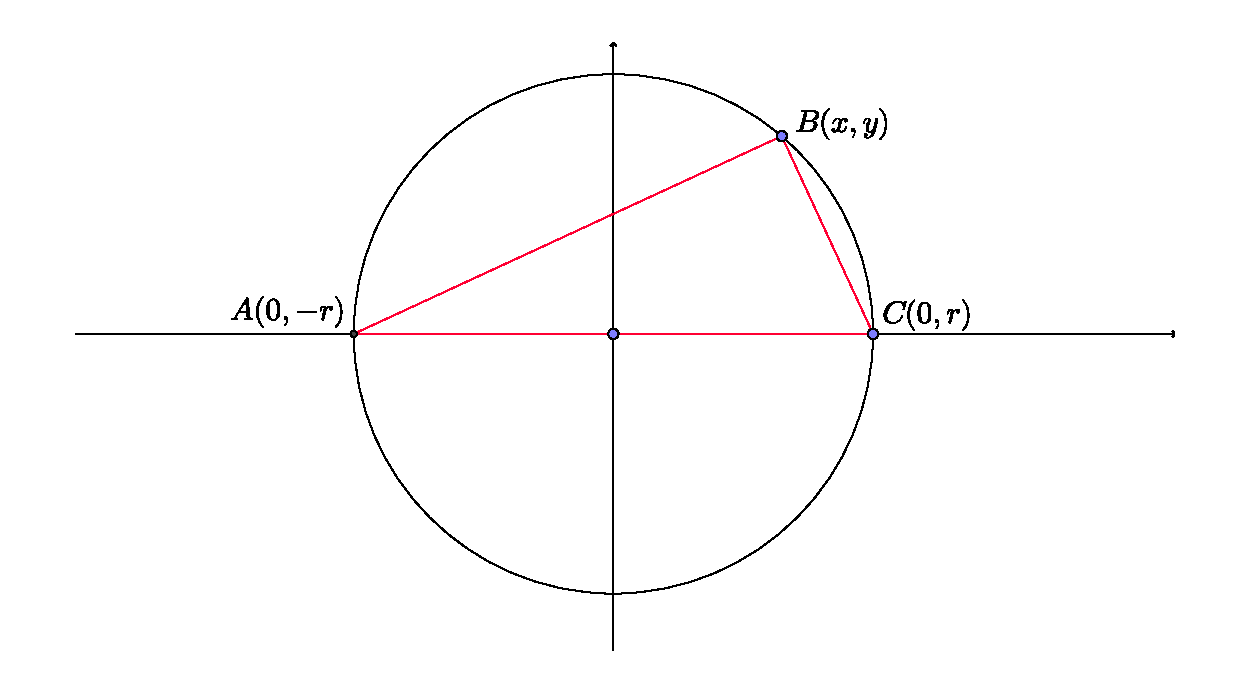
\includegraphics[scale=0.5]{circle.pdf}
\end{center}

\begin{enumerate}

\item By first expressing the circle as two separate explicit functions of $x$, compute the slope of the tangent line to the circle at each point where $x=1$.

\includegraphics[scale=0.5]{start.pdf}
{{$\left.\frac{dy}{dx}\right|_{(x,y)=\left(1,\sqrt{3}\right)}=-\frac{1}{\sqrt{3}}$ and $\left.\frac{dy}{dx}\right|_{(x,y)=\left(1,-\sqrt{3}\right)}=\frac{1}{\sqrt{3}}$}}
\includegraphics[scale=0.5]{end.pdf}


\item By using implicit differentiation, compute the slope of the tangent line to the circle at each point where $x=1$.

\includegraphics[scale=0.5]{start.pdf}
{{$\left.\frac{dy}{dx}\right|_{(x,y)=\left(1,\sqrt{3}\right)}=-\frac{1}{\sqrt{3}}$ and $\left.\frac{dy}{dx}\right|_{(x,y)=\left(1,-\sqrt{3}\right)}=\frac{1}{\sqrt{3}}$}}
\includegraphics[scale=0.5]{end.pdf}


\item Find the point of intersection of the lines which are tangent to the circle when $x=1$.

\includegraphics[scale=0.5]{start.pdf}
{{$(4,0)$}}
\includegraphics[scale=0.5]{end.pdf}


\end{enumerate}

\end{enumerate}

\noindent {\bf For problems 4-8, use implicit differentiation to find $\frac{dy}{dx}$.}

\begin{enumerate}
\setcounter{enumi}{3}

\item $x^2y=9$ 

\includegraphics[scale=0.5]{start.pdf}
{{$\frac{dy}{dx}=\frac{-2y}{x}$}}
\includegraphics[scale=0.5]{end.pdf}


\item $xy^2+y^3 = 6$ 

\includegraphics[scale=0.5]{start.pdf}
{{$\frac{dy}{dx}=\frac{-y}{2x+3y}$}}
\includegraphics[scale=0.5]{end.pdf}


\item $\frac{1-y^2}{1-2x}=x$ 

\includegraphics[scale=0.5]{start.pdf}
{{$\frac{dy}{dx}=\frac{4x-1}{2y}$}}
\includegraphics[scale=0.5]{end.pdf}


\item $y\cos{x} + y^2x = 3x$ 

\includegraphics[scale=0.5]{start.pdf}
{{$\frac{dy}{dx}=\frac{3-y^2+y\sin{x}}{2xy+\cos{x}}$}}
\includegraphics[scale=0.5]{end.pdf}


\item $x^2+y^3=10$ 

\includegraphics[scale=0.5]{start.pdf}
{{$\frac{dy}{dx}=\frac{-2x}{3y^2}$}}
\includegraphics[scale=0.5]{end.pdf}


\end{enumerate}

\noindent {\bf For problem 9-10, compute $\frac{d^2y}{dx^2}$ in terms of $x$ and $y$}

\begin{enumerate}
\setcounter{enumi}{8}

\item $2x^2-3y^2=4$

\includegraphics[scale=0.5]{start.pdf}
{{$\frac{d^2y}{dx^2}=-\frac{8}{9y^3}$}}
\includegraphics[scale=0.5]{end.pdf}


\item $y+\sin{y}=x$

\includegraphics[scale=0.5]{start.pdf}
{{$\frac{d^2y}{dx^2}=\frac{\sin{y}}{(1+\cos{y})^3}$}}
\includegraphics[scale=0.5]{end.pdf}


\end{enumerate}

\noindent {\bf For problems 11-12, find the equation of the line tangent to the curve at the given point.}

\begin{enumerate}
\setcounter{enumi}{10}

\item $x^2+y^2 = 10$ at $(1,3)$ 

\includegraphics[scale=0.5]{start.pdf}
{{$y=\frac{-x}{3}+\frac{10}{3}$}}
\includegraphics[scale=0.5]{end.pdf}


\item $\frac{1-xy}{1-5x}=2x$ at $(1,9)$ 

\includegraphics[scale=0.5]{start.pdf}
{{$y=9x$}}
\includegraphics[scale=0.5]{end.pdf}


\item Consider the ellipse given by $\frac{x^2}{a^2}+\frac{y^2}{b^2}=1$, where $a$ and $b$ are positive real numbers.  Use implicit differentiation to compute the slope of the line which is tangent to the curve at $(x_0,y_0)$.

\includegraphics[scale=0.5]{start.pdf}
{{$\left.\frac{dy}{dx}\right|_{(x,y)=(x_0,y_0)}=-\frac{b^2x_0}{a^2y_0}$}}
\includegraphics[scale=0.5]{end.pdf}


\item The set of ordered pairs $(x,y)$ which satisfy the equation $(x^2+y^2-x)^2=x^2+y^2$ form the curve shown below, called a \underline{cardioid}.

\begin{center}
\includegraphics[scale=0.5]{cardioid.pdf}
\end{center}

Let $L_1$ be the line which is tangent to the curve at the point $(0,1)$ and let $L_2$ be the line which is tangent to the curve at the point $(0,-1)$.  At which point in the $xy$-plane do $L_1$ and $L_2$ intersect?

\includegraphics[scale=0.5]{start.pdf}
{{$(-1,0)$}}
\includegraphics[scale=0.5]{end.pdf}


\newpage

\item The curve below is the graph of $(x^2+y^2-1)^3-x^2y^3=0$.

\begin{center}
\includegraphics[scale=0.5]{heart}
\end{center}

\begin{enumerate}

\item Sketch the tangent line to to graph at the point $(-1,1)$.

\includegraphics[scale=0.5]{start.pdf}
{{\includegraphics[scale=.3]{Heart_Tangent.pdf}}}
\includegraphics[scale=0.5]{end.pdf}


\item Find an equation of line which is tangent to the graph at the point $(-1,1)$.\\
\underline{Pro-tip:} Plug in $(-1,1)$ after applying $\frac{d}{dx}$ to both sides of the equation but before solving for $\frac{dy}{dx}$.

\includegraphics[scale=0.5]{start.pdf}
{{$y=\frac{4}{3}x+\frac{7}{3}$}}
\includegraphics[scale=0.5]{end.pdf}


\end{enumerate}

\end{enumerate}

\end{document}